%
%Не забыть:
%--------------------------------------
%Вставить колонтитулы, поменять название на титульнике



%--------------------------------------

\documentclass[a4paper, 12pt]{article} 

%--------------------------------------
%Russian-specific packages
%--------------------------------------
%\usepackage[warn]{mathtext}
\usepackage[T2A]{fontenc}
\usepackage[utf8]{inputenc}
\usepackage[english,russian]{babel}
\usepackage[intlimits]{amsmath}
\usepackage{esint}
%--------------------------------------
%Hyphenation rules
%--------------------------------------
\usepackage{hyphenat}
\hyphenation{ма-те-ма-ти-ка вос-ста-нав-ли-вать}
%--------------------------------------
%Packages
%--------------------------------------
\usepackage{amsmath}
\usepackage{amssymb}
\usepackage{amsfonts}
\usepackage{amsthm}
\usepackage{latexsym}
\usepackage{mathtools}
\usepackage{etoolbox}%Булевые операторы
\usepackage{extsizes}%Выставление произвольного шрифта в \documentclass
\usepackage{geometry}%Разметка листа
\usepackage{indentfirst}
\usepackage{wrapfig}%Создание обтекаемых текстом объектов
\usepackage{fancyhdr}%Создание колонтитулов
\usepackage{setspace}%Настройка интерлиньяжа
\usepackage{lastpage}%Вывод номера последней страницы в документе, \lastpage
\usepackage{soul}%Изменение параметров начертания
\usepackage{hyperref}%Две строчки с настройкой гиперссылок внутри получаеммого
\usepackage[usenames,dvipsnames,svgnames,table,rgb]{xcolor}% pdf-документа
\usepackage{multicol}%Позволяет писать текст в несколько колонок
\usepackage{cite}%Работа с библиографией
\usepackage{subfigure}% Человеческая вставка нескольких картинок
\usepackage{tikz}%Рисование рисунков
\usepackage{float}% Возможность ставить H в положениях картинки
% Для картинок Моти
\usepackage{misccorr}
\usepackage{lscape}
\usepackage{cmap}



\usepackage{graphicx,xcolor}
\graphicspath{{Pictures/}}
\DeclareGraphicsExtensions{.pdf,.png,.jpg}

%----------------------------------------
%Список окружений
%----------------------------------------
\newenvironment {theor}[2]
{\smallskip \par \textbf{#1.} \textit{#2}  \par $\blacktriangleleft$}
{\flushright{$\blacktriangleright$} \medskip \par} %лемма/теорема с доказательством
\newenvironment {proofn}
{\par $\blacktriangleleft$}
{$\blacktriangleright$ \par} %доказательство
%----------------------------------------
%Список команд
%----------------------------------------
\newcommand{\grad}
{\mathop{\mathrm{grad}}\nolimits\,} %градиент

\newcommand{\diver}
{\mathop{\mathrm{div}}\nolimits\,} %дивергенция

\newcommand{\rot}
{\ensuremath{\mathrm{rot}}\,}

\newcommand{\Def}[1]
{\underline{\textbf{#1}}} %определение

\newcommand{\RN}[1]
{\MakeUppercase{\romannumeral #1}} %римские цифры

\newcommand {\theornp}[2]
{\textbf{#1.} \textit{ #2} \par} %Написание леммы/теоремы без доказательства

\newcommand{\qrq}
{\ensuremath{\quad \Rightarrow \quad}} %Человеческий знак следствия

\newcommand{\qlrq}
{\ensuremath{\quad \Leftrightarrow \quad}} %Человеческий знак равносильности

\renewcommand{\phi}{\varphi} %Нормальный знак фи

\newcommand{\me}
{\ensuremath{\mathbb{E}}}

\newcommand{\md}
{\ensuremath{\mathbb{D}}}



%\renewcommand{\vec}{\overline}




%----------------------------------------
%Разметка листа
%----------------------------------------
\geometry{top = 3cm}
\geometry{bottom = 2cm}
\geometry{left = 1.5cm}
\geometry{right = 1.5cm}
%----------------------------------------
%Колонтитулы
%----------------------------------------
\pagestyle{fancy}%Создание колонтитулов
\fancyhead{}
%\fancyfoot{}
%\fancyhead[R]{\textsc{Получение и измерение вакуума}}%Вставить колонтитул сюда
%----------------------------------------
%Интерлиньяж (расстояния между строчками)
%----------------------------------------
%\onehalfspacing -- интерлиньяж 1.5
%\doublespacing -- интерлиньяж 2
%----------------------------------------
%Настройка гиперссылок
%----------------------------------------
\hypersetup{				% Гиперссылки
	unicode=true,           % русские буквы в раздела PDF
	pdftitle={Заголовок},   % Заголовок
	pdfauthor={Автор},      % Автор
	pdfsubject={Тема},      % Тема
	pdfcreator={Создатель}, % Создатель
	pdfproducer={Производитель}, % Производитель
	pdfkeywords={keyword1} {key2} {key3}, % Ключевые слова
	colorlinks=true,       	% false: ссылки в рамках; true: цветные ссылки
	linkcolor=blue,          % внутренние ссылки
	citecolor=blue,        % на библиографию
	filecolor=magenta,      % на файлы
	urlcolor=cyan           % на URL
}
%----------------------------------------
%Работа с библиографией (как бич)
%----------------------------------------
\renewcommand{\refname}{Список литературы}%Изменение названия списка литературы для article
%\renewcommand{\bibname}{Список литературы}%Изменение названия списка литературы для book и report
%----------------------------------------
\begin{document}
	\begin{titlepage}
		\begin{center}
			$$$$
			$$$$
			$$$$
			$$$$
			% To be reworked
			{\Large{НАЦИОНАЛЬНЫЙ ИССЛЕДОВАТЕЛЬСКИЙ УНИВЕРСИТЕТ}}\\
			\vspace{0.1cm}
			{\Large{ВЫСШАЯ ШКОЛА ЭКОНОМИКИ}}\\
			\vspace{0.25cm}
			{\large{Факультет физики}}\\
			\vspace{4cm}
			{\Huge\textbf{{Лабораторная работа}}}\\%Общее название
			\vspace{1cm}
			{\LARGE{<<Метод качания. Определение периодов идентичности по рентгенограмме монокристалла. Индицирование рефлексов>>}}\\%Точное название
			\vspace{2cm}
			{Работу выполнил студент 3 курса}\\
			{Захаров Сергей Дмитриевич}
			\vfill
			
\includegraphics[width=0.2\linewidth]{HSElogo}
			\vfill
			Москва\\
			2020
		\end{center}
	\end{titlepage}

\tableofcontents

\newpage

\section{Анализ рентгенограммы}

Для выполнения работы была взята рентгенограмма, представленная на рисунке \ref{fig:rentgen}.

\begin{figure}[H]
	\centering
	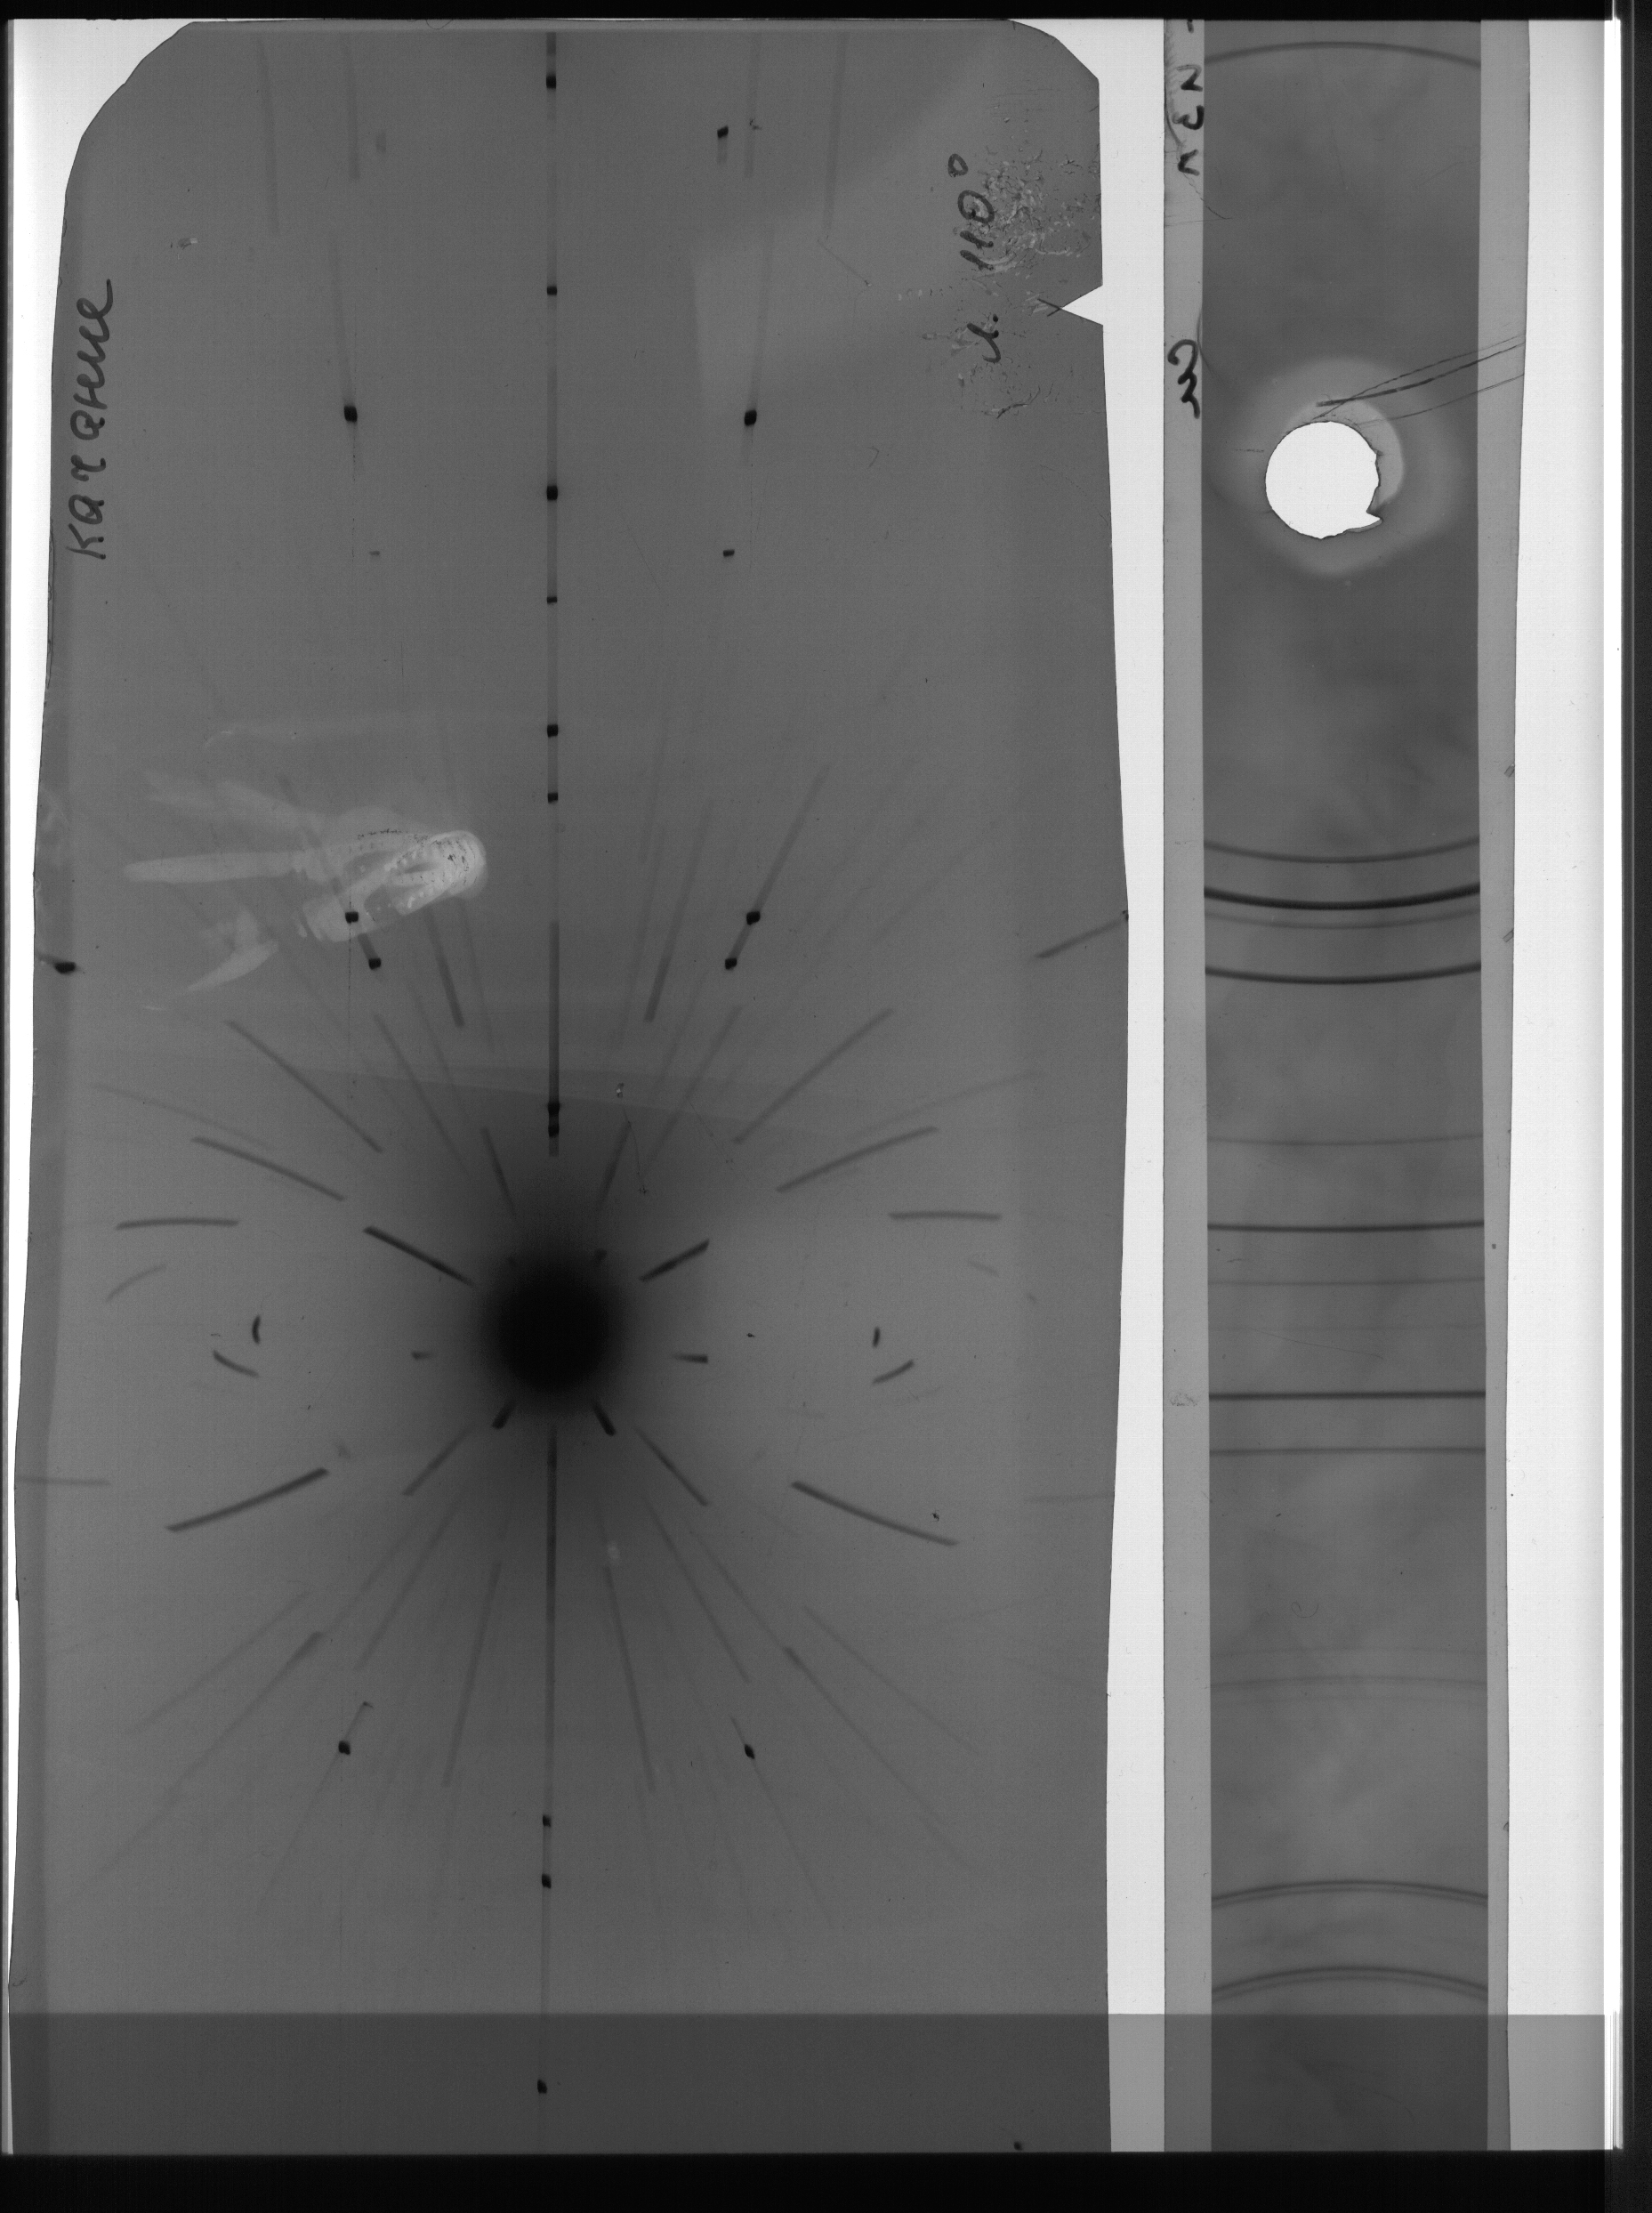
\includegraphics[angle=-90, width=0.9\linewidth]{3a}
	\caption{Рентгенограмма для анализа (сверху)}
	\label{fig:rentgen}
\end{figure}

На основании представленной рентгенограммы можем заявить, что присутствуют $\alpha$- и $\beta$-рефлексы, видно две первых слоевых линии, симметричных относительно нулевой слоевой линии.

Появление слоевых линий объясняется с помощью построения Эвальда, демонстрирующего принцип их появления при вращении (см. рисунок \ref{fig:Evald_ex}).

\begin{figure}[H]
	\centering
	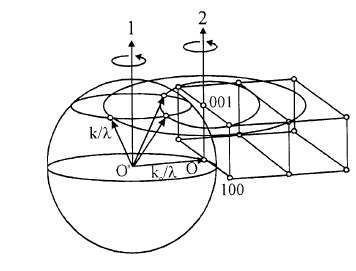
\includegraphics[width=0.7\linewidth]{Evald_ex}
	\caption{Построение Эвальда, объясняющее происхождение слоевых линий на рентгенограмме вращения (Рис. 4.2а \cite{Practicum}). Здесь 1 --- ось вращения кристалла и ось кассеты с пленкой, 2 --- ось вращения обратной решетки.}
	\label{fig:Evald_ex}
\end{figure}

\section{Определение направления качания}

Согласно методике, изложенной в \cite{Practicum}, для определения периода идентичности возможно использовать формулу

\begin{equation}
	J_{mnp} = n \lambda \sqrt{1 + \left(\frac{R}{l_n}\right)}
	\label{eq:J}
\end{equation}

Здесь $R$ --- радиус камеры, $l_n$ --- расстояние от нулевой до $n$-ной слоевой линии, $\lambda$ --- длина волны излучения. Известно, что в работе использовалась камера РКВ с цилиндрической кассетой, значит $R = 43$~мм.

После анализа рентгенограммы было установлено, что $l_1 = 19.09$~ммКроме того, для используемого излучения $\lambda_\alpha = 1.54178$~\AA. Поэтому из (\ref{eq:J}) получаем:

\begin{equation}
	 \boxed{J = 3.83 \text{ \AA}}
\end{equation}

Нам известно, что в работе использовался кристалл кремния, для которого $a \approx 5.4307$~\AA. С учетом полученных нами данных, можем заключить, что имеется связь:

\begin{equation}
	\frac{a}{\sqrt{2}} \approx J
\end{equation}

Из этого, в свою очередь, заключаем, что направление на узловую прямую соответствует~[110].

\section{Индицирование рефлексов на нулевой слоевой линии}

Для определения межплоскостного расстояния (и дальнейшего индицирование рефлексов) возможно использование условию Брэгга--Вульфа:

\begin{equation}
	2 d \sin\theta = n\lambda
\end{equation}

Здесь $d$ --- межплоскостное расстояние, $\theta$ --- брэгговский угол, $n$ --- порядок дифракционного максимума (рефлекса), $\lambda$ --- длина волны.

Как уже было сказано, в лабораторной использовалась камера РКВ с цилиндрической кассетой. Это означает, что угол $\theta$ можно измерять, по расстоянию $l$ от центра рентгенограммы до соответствующего рефлекса (на нулевой слоевой линии) при условии, что $l$ измеряется в миллиметрах: 

\begin{equation}
	\theta = \frac{l}{1.5}
\end{equation}

Мы также предполагаем, что видим первый порядок дифракции, а значит $n = 1$.

Все получаемые в ходе лабораторной данные будем вносить в одну сводную таблицу.

На основании рентгенограммы мы можем примерно определить, какие рефлексы принадлежат к $\beta$, а какие к $\alpha$ (по тому, есть ли соответствующий рефлекс чуть ниже первой слоевой линии, см. рисунок 4.4 в \cite{Practicum}). Для того, чтобы это подтвердить, или опровергнуть, посчитаем $\sin\theta_\beta$ аналогично тому, как это было сделано в Лабораторной 1. С учетом того, какое излучение используется, сразу выпишем:

\begin{align}
	\lambda_\alpha = 1.54178 \text{ \AA} \\
	\lambda_\beta = 1.39217 \text{ \AA}
\end{align}

В расчетных формулах для $\beta$- и $\alpha$-рефлексов будем использовать $\lambda_\beta$ и $\lambda_\alpha$ соответственно. С учетом этого запишем в таблицу $d$.

Индексы $hkl$ определим с учетом наличия квадратичной формы, которая связывает $d$ и $hkl$, которая выражается следующим образом:

\begin{equation}
	\frac{1}{d^2} = \frac{h^2 + k^2 + l^2}{a^2} \qrq h^2 + k^2 + l^2 = \frac{a^2}{d^2}
\end{equation}

В качестве дополнительного условия на индексы поймем следующее: в силу того, что качание, согласно первому пункту лабораторной, проводилось вокруг оси [110], получим:

\begin{equation}
	mh + nk + pl = h + k = 0 \qrq h = -k
\end{equation} 

Здесь $m, n, k$ --- числа в записи оси $[mnk] = [110]$.

Поэтому мы должны искать рефлексы вида $(h, -h, l)$

\begin{table}[H]
	\centering
	\begin{tabular}{|c|c|c|c|c|c|c|c|c|}
		\hline
		$N$ & $l$, мм & $\theta$ & $\sin\theta$ & $\sin\theta_\beta$ & $\alpha$/$\beta$ & $d$ & $\sum\limits_i h_i^2$ & $hkl$ \\
		\hline
		1 & 19.56 & 13.04 & 0.23 & 0.20 & $\beta$ & 3.09 & 3.1 & 1-11 \\
		\hline
		2 & 21.84 & 14.56 & 0.25 & 0.23 & $\alpha$ & 3.07 & 3.13 & 1-11 \\
		\hline
		3 & 51.22 & 34.15 & 0.56 & 0.51 & $\beta$ & 1.24 & 19.18 & 3-31 \\
		\hline
		4 & 57.57 & 38.38 & 0.62 & 0.56 & $\alpha$ & 1.24 & 19.13 & 3-31 \\
		\hline
		5 & 69.93 & 46.62 & 0.73 & 0.66 & $\beta$ & 0.96 & 32.15 & 4-40 \\
		\hline
		6 & 80.09 & 53.39 & 0.80 & 0.72 & $\alpha$ & 0.96 & 31.98 & 4-40 \\
		\hline
		7 & 99.31 & 66.21 & 0.92 & 0.83 & $\alpha?$ & 0.84 & 41.55 & 541? \\
		\hline
		8 & 119.2 & 79.47 & 0.98 & 0.89 & $\alpha$ & 0.78 & 47.97 & 4-44 \\
		\hline
	\end{tabular}
\end{table}

Сравнивая результат с имеющимися в общем доступе базам данных (например, с помощью Match), становится понятно, что сошлись все рефлексы, кроме одного (седьмого), который в таблице указан со знаком вопроса (поскольку как минимум не подчиняется установленному нами виду рефлексов). Предположительно он может быть бета-рефлексом от какой-то более сильной альфы, находящейся дальше, но проверить это в данной лабораторной возможным не представляется.

\section{Чертеж узловой плоскости ОР, соответствующей нулевой слоевой линии. Поиск узлов, пересекающих сферу отражения при качании кристалла}

Как известнор, обратной решетке должны соответствовать целочисленные узлы координатной сетки. Для соответствующего построения сперва посчитаем радиус сферы Эвальда в нашем масштабе (учтя, что в нашем масштабе единичный отрезок есть $1/a$):

\begin{equation}
	R = \frac{a}{\lambda} \approx 3.522
	\label{eq:R}
\end{equation}

Качание кристалла происходило вокруг оси [110], что было установлено в 1-ом пункте лабораторной. По этой причине кажется логичным, что центр сферы должен лежать на прямой $y=x$. Кроме того, сфера должна касаться начала координат. Этих условий в купе с радиусом, посчитанным в (\ref{eq:R}), достаточно для однозначного ее рисования. Для того, чтобы не делать это совсем уж ''на глазок'', воспользуемся современными программами.

После того, как сфера была нарисована, в соответствии с представленными данными повернем ее вокруг начала координат на $15^\circ$ в обе стороны, получив таким образом красную и синюю окружности на  рис. \ref{fig:Evald}.

После этого, наконец, расположим посчитанные нами рефлексы в тех же самых координатах. Как видно, все они лежат в пределах заметаемой области (рефлекс с индексами (541) было решено не приводить в силу его неоднозначной трактовки).

\begin{figure}[H]
	\centering
	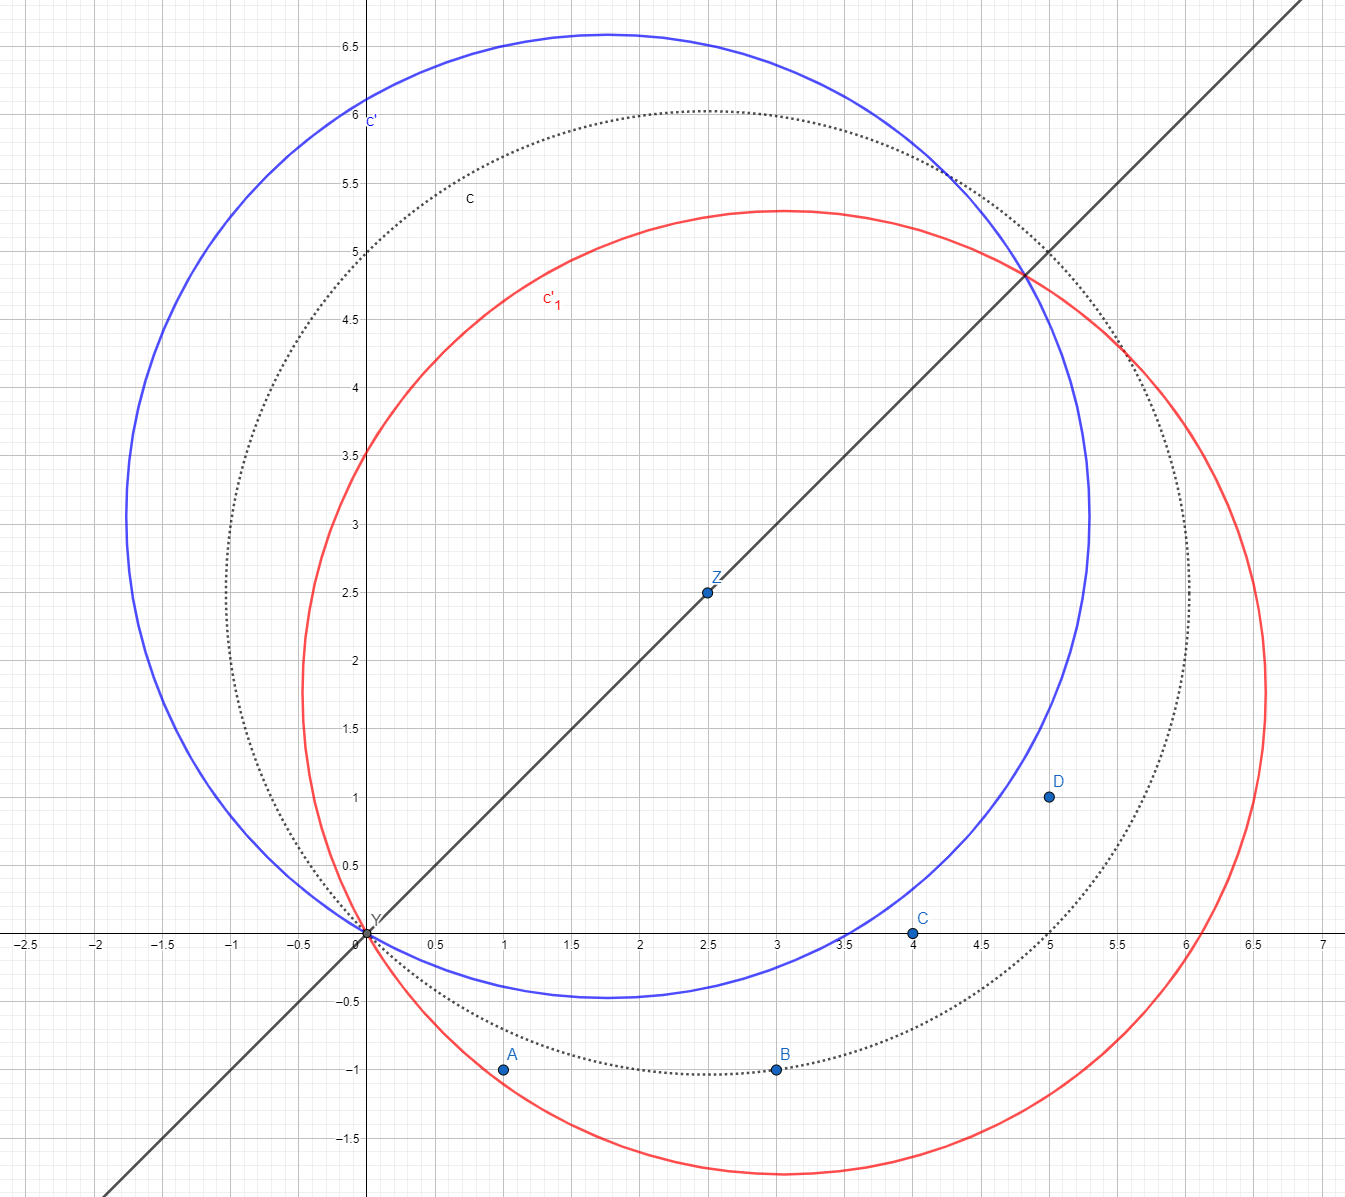
\includegraphics[width=0.9\linewidth]{Evald}
	\caption{К построению сферы Эвальда}
	\label{fig:Evald}
\end{figure}

\section{Вывод}

Вместо заключения приведем ряд фактов, установленных в ходе экспериментов, а также подытожим сделанное:

\begin{enumerate}
	\item Период идентичности на оси кристалла составил $J = 3.83$~\AA. Сравнив полученное значение с $a = 5.4307$\AA, было выдвинуто предположение, что направление качания есть [110].
	
	\item Были проиндицированы рефлексы на нулевой слоевой линии. Полученные индексы за одним исключением сошлись с имевшейся в наличии базе данных для кристалла кремния.
	
	\item Было совершено построение Эвальда, подтвердившее возможность появления рефлексов с этими индексами при качании кристалла вокруг указанной оси на $15^\circ$.
\end{enumerate}


\newpage

\begin{thebibliography}{1}
	\bibitem{Practicum}
	Рентгендифракционные методы изучения структуры монокристаллов, поликристаллических и аморфных материалов
\end{thebibliography}




\end{document}